\documentclass[uplatex,dvipdfmx]{jsarticle}

\usepackage[uplatex,deluxe]{otf} 
\usepackage[noalphabet]{pxchfon} 
\usepackage{stix2} 
\usepackage[fleqn,tbtags]{mathtools} 
\usepackage{amsmath}
\usepackage{url}
\usepackage{float} 

\setcounter{tocdepth}{3}
\usepackage{moreverb}
\usepackage{lscape}
\usepackage{ascmac}
\usepackage{xurl}
\usepackage{graphicx} % 画像挿入用

\begin{document}

\title{危険交差点警告システム}
\author{25G1051 近藤巧望}
\maketitle

\section{はじめに}

\subsection{社会的背景}
自転車は温室効果ガスを排出しない移動手段であり,環境に優しい交通手段として注目されている.
日本の自転車保有台数は約6870万台(つまり約二人に1台)となっており,交通渋滞の緩和や健康促進,
地球温暖化等の環境問題への配慮の観点から,政府も自転車活用推進法に基づき自転車の利用を推奨している
\cite{ref:koutuusyou_1,ref:koutuusyou_2}.

しかし交通事故に焦点を当てると,自転車搭乗中の出会い頭衝突事故は2023年時点で全体の52.9\%と,
自転車事故の中で最も多く発生している事故であり,深刻な問題となっている\cite{ref:sonpo_1}.
自転車事故は特に交差点で発生することが多く,視界が遮られたり信号の認識が困難だったりするため,事故が起こりやすい.

従来の交通事故対策として交通安全教育や,道路交通法といった法規制がある.
しかし,これらの対策だけでは,利用者の多様な判断・行動パターンや道路上での様々な危険的要因に十分に適応し,事故の発生を根本的に解決することは困難である.
例えば,交通安全教育は安全意識の向上に寄与するが,交通安全教育では即時性がなく交通ルールなどの知識が形骸化してしまうことから,
すべての自転車利用者が常に高い安全意識を持って行動することが保証できない.
法規制の強化についても利用者の行動変容を促すには限界があり,瞬間的な判断が求められる交差点での事故防止には,
さらに直接的かつ即時的な対策が必要である.

以上のことから,従来の交通安全教育や法規制に加えて,技術的な新しい事故防止策が求められる.
特に,リアルタイムで危険を検知し利用者に警告するようなシステムは個々の利用者の安全意識に依存せず客観的な危険情報を提供することで,
従来の交通安全教育や法規制の限界を補完するという形で事故率を低減させる可能性をもっている.

\subsection{問題点}
既存のリアルタイム検知システムとして,自動車向けのナビゲーションでの事故多発エリアの警告システムがある.

このシステムは,GNSS(Global Navigation Satellite System),地図データ,事故多発エリアのデータベース,これらをもとに警告するかを判定するソフトウェアで主に構成されている.
事故多発エリアに近づくと音声で警告を行うことで,運転者の注意力を高め,事故の発生を防止することを目的としているが,
自動車の通りが少ない地域などでは事故データの不足により警告の判定の正確性が低下する可能性がある.
また,道路の改良などで事故多発エリアの状況が変化した場合,データベースの更新が遅れると,実際の危険性と警告内容に乖離が生じる可能性がある.
これらのことから,自動車向けの事故多発エリア警告システムのような技術を自転車へ同様に導入したとしても,事故データに依存することから地域や環境に性能が左右されてしまうため,広範囲で適用できるとは限らないという問題が生じる.

実際に,既存の自動車向け衝突防止システムADAS(Advanced Driver-Assistance Systems)は,
警告や自動ブレーキによって使用者の安全を守るシステムとして知られているが,
先行研究では,衝突事故の事故事例の少なさから,有意な結果が得られなかった\cite{ref:adas}.
つまり,ADASのようなシステムは,事故データに依存することから,事故データが不足している地域では効果が限定的になる可能性がある.

\subsection{目的}
本提案の目的は,自転車での出会い頭衝突を防ぐための対策を考え,自転車事故による負傷者や死者数を減少させることである.
具体的には,自転車での出会い頭衝突の事故を現状から約10\%削減させることを目指す.
令和6年中の自転車関連事故全体の件数が67,531件であることから,全体の52.9\%にあたる出会い頭衝突の事故件数が約35,700件であることを考慮すると,
約3,570件の事故を削減することができると考えられる.

目標値を10\%に設定した理由として,
前述のADASでは,衝突事故を10\%削減することに成功したという事例が報告されている\cite{ref:adas_purpose}.
しかし,有意な結果が得られなかったことから,ADASで成功した10\%の削減を本提案により更に現実的なものにしたいと考えている.

さらに,地域や環境に性能が左右されてしまう現状の対策として,AI(Artificial Intelligence)を用いた画像認識技術を活用することで,事故データに依存しないシステムを構築する.
それにより,偏った事故データに依存することなく,より柔軟な危険検知が可能になり,地域や環境に関係なく広範囲で適用できるシステムを実現できると考えられる.
本提案により,従来のシステムよりも更に広域で性能が発揮でき,子どもから高齢者まで幅広い年齢層の自転車搭乗者が安全に自転車を利用できる環境の整備に貢献することを目指す.

\section{解決策としての提案手法}

\subsection{提案手法の概要}
本システムは,アプリケーションとして導入し,スマートフォンと連携することで,ユーザーに対してリアルタイムで危険情報を提供する.
本提案では,日本が運用するGNSS(Global Navigation Satellite System)であるGPS(Global Positioning System)とQZSS(Quasi-Zenith Satellite System)を用いて使用者の位置情報を取得し,Google Maps Static APIを用いて現在地周辺の道路の航空画像を取得する.
その後,AIによる画像認識技術を用いて交差点を検出し,危険性が高い交差点が検出された場合は搭乗者に音声とバイブレーションで警告を行う.

使用時は,スマートフォンにアプリケーションをインストールし,GNSS機能を有効にした状態でアプリケーションを起動する.
そして固定具で自転車のハンドルに取り付けて使用する.

\subsection{提案手法の構成要素について}

\begin{table}[H]
  \centering
  \caption{システムの構成要素}
  \label{tab:system_components}
  \begin{tabular}{|c|l|l|}
    \hline
    項目 & 構成要素 & 備考\\ \hline
    1 & スマートフォンGNSS & 位置情報を取得するためのGNSS機能(GPSとQZSSを使用) \\ \hline
    2 & Google Maps Static API & 現在地周辺の航空画像を取得 \\ \hline
    3 & 画像認識モデル & 画像の分類・危険な交差点を検出 \\ \hline
    4 & 警告システム & 搭乗者に音声とバイブレーションで警告を行う \\ \hline
  \end{tabular}
\end{table}

\begin{figure}[H]
  \centering
  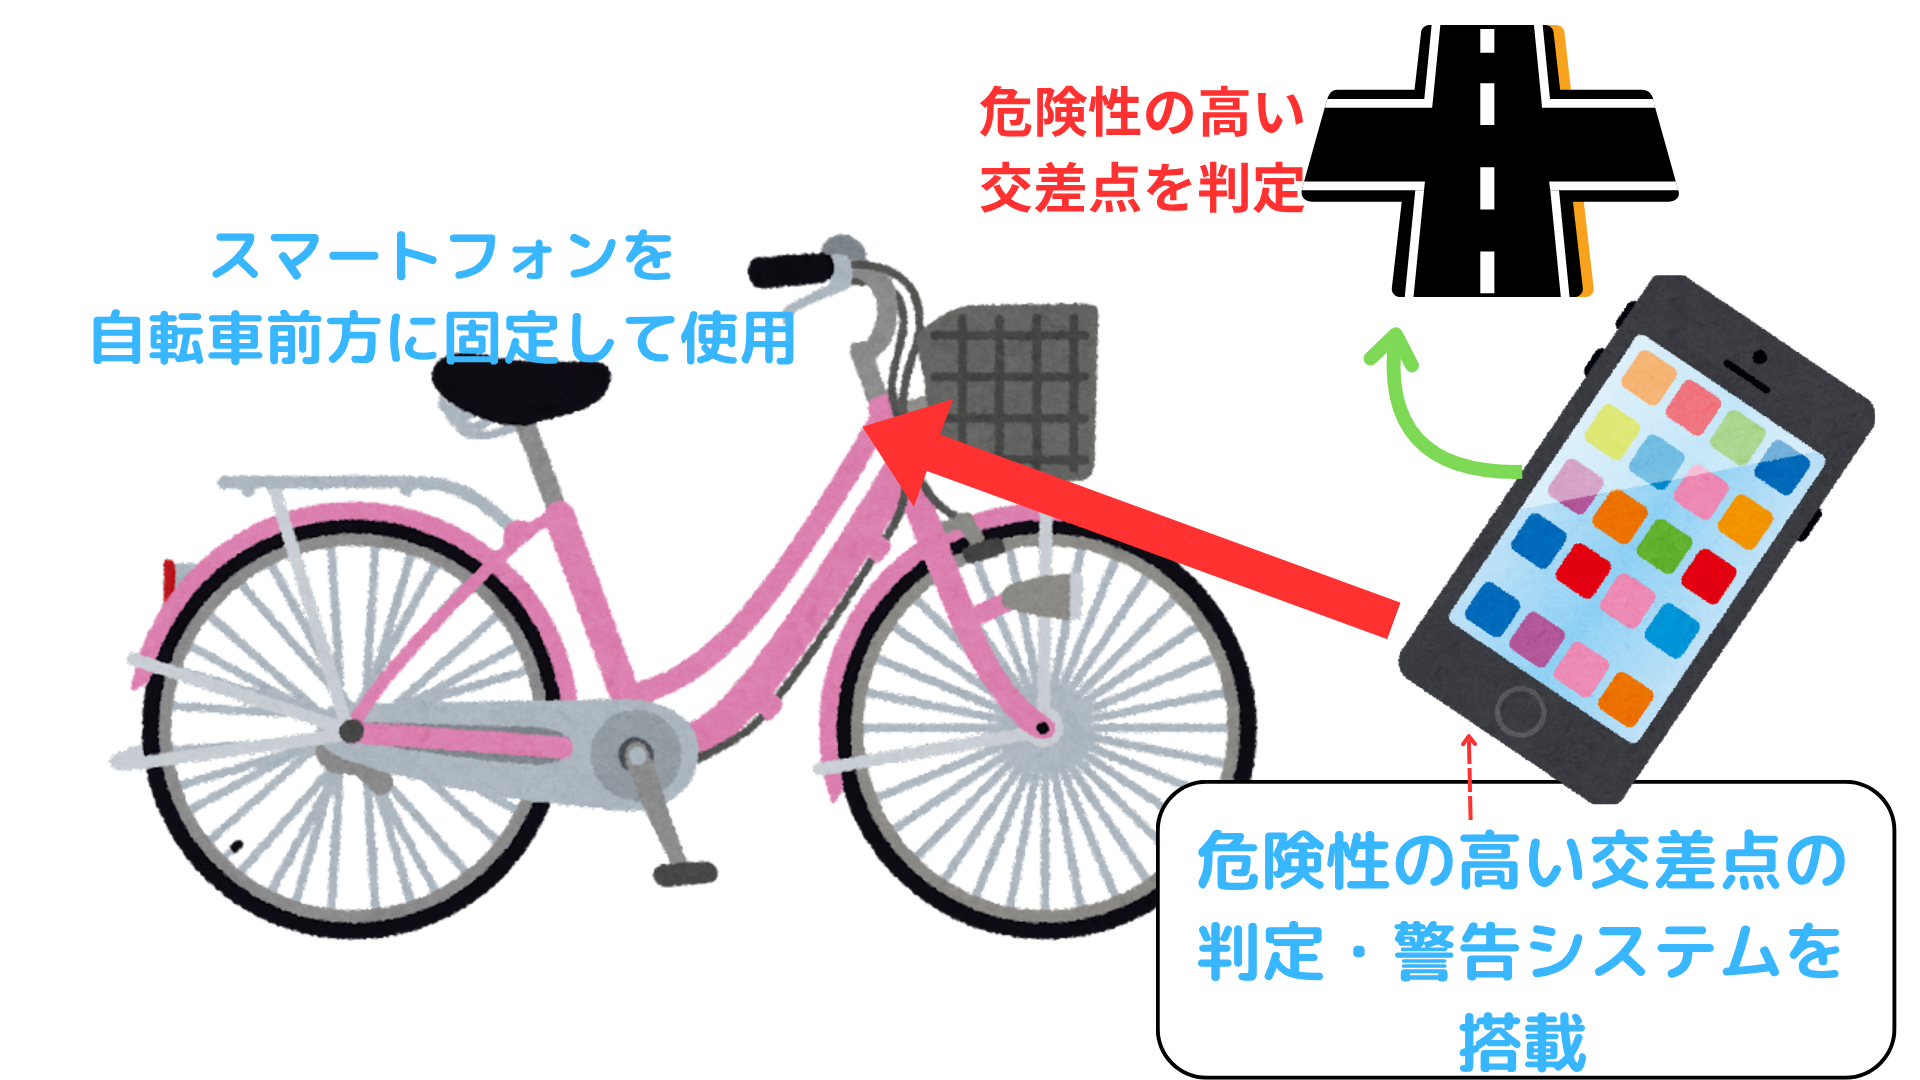
\includegraphics[width=14cm]{./Figs/gainenzu_final.png}
  \caption{危険交差点警告システムの概念図}
  \label{fig:idea}
\end{figure}

システムの構成要素を表1に,システムの概念図を図1に示す.
本システムは主に4つの要素から構成される.

まず,使用者の位置情報を取得するためのGNSSである.
本提案では,QZSSとGPSを併用するが,QZSSとは日本国内で運用されている衛星測位システムであり,主に日本とアジア太平洋地域の任意の地点で正確な位置情報を,人工衛星からスマートフォンで受け取ることができる.
スマートフォンの内部にはGPS(Global Positioning System)とQZSSに対応したGNSS受信モジュールが搭載されているため,GPSだけでは不十分な点を補う形でQZSSを併用することで,より正確な位置情報を取得できる.
GPSのみの使用に限定してしまうと,都市部のビル街や山間部で衛星が遮蔽されやすく補足数が減るのに加え,マルチパスによって誤差が大きくなる可能性がある.
対してQZSSは,GPSと比べて日本国内での測位精度が高いことが知られている他,
QZSSは日本の天頂付近を通過するように設計されているため,都市部の高層ビル街や山間部などでの受信性能が向上するという利点がある\cite{ref:qzss}.
しかし,衛星数が2025年時点で4機と少なく,単独での測位には限界があるため,GPSと併用することで,より安定した位置情報の取得が可能になる.
以上の理由から,本提案ではGPSとQZSSを併用することにした.
これらのGNSSを用いることで,使用者の正確な位置情報をリアルタイムで取得することができ,
使用者の位置情報は,航空画像の取得範囲を特定するために使われる.

次に,Google Maps Static APIを用いて使用者の周辺の交差点情報を取得する.
Google Maps Static API とは,Google が提供する地図画像を取得するための API(Application Programming Interface) であり,
航空写真や地図画像を取得することができる.
Google Maps Static APIは,URLにパラメータを指定するだけで簡単に地図画像を取得できるうえに使用するための料金に無料枠があることから,
扱いやすさとコスト面で優れている.
また,ドキュメントが豊富で導入が容易であることも採用理由の一つである.
同じく地図を表示させるAPIとしてGoogle Maps JavaScript APIがあるが,Google Maps Static APIはデータの読み込み量が少ないという点でも優れている.
Google Chromeのデベロッパー ツールを用いてGoogle Maps Static APIとGoogle Maps JavaScript API双方の公式サンプルページにおけるデータ転送量を確認したところ,
Google Maps Static APIはデータの読み込み量が63.8 kB,Google Maps JavaScript APIはデータの読み込み量が433 kBであり,
約7倍の差があった\cite{ref:developer_static,ref:developer_js}.Google Maps Static APIは静的な画像を取得するのに対し,Google Maps JavaScript APIは動的に地図を表示するため,
ほぼ単一な画像サイズと同じデータ量であるGoogle Maps Static APIの方が,地図表示プログラム一式を読み込むGoogle Maps JavaScript APIよりもデータの読み込み量が少なくなり,
通信速度が高速である.
本システムは高速なリアルタイム処理が求められるため,データの読み込み量が少ないGoogle Maps Static APIがより適している.

画像認識モデルは,機械学習により画像から危険な交差点を検出する.
道路の形状から交差点を判定し,さらに形状・塀・街路樹などの障害物から危険度を分類する.
危険度によって道路を分類することで,すべての交差点に近づくたびに作動することを防ぎ,必要な場合のみ警告を行う.

警告の作動タイミングについては,交差点の手前約16mで警告を行う.
搭乗者が警告に気づいてからブレーキをかけるまでの距離(以下,空走距離)は,一般的な自転車の移動速度時速約15km(秒速約4.2m)を加味し,
搭乗者が警告を受けてから行動に移すまでの時間を少し余裕を見て1.5秒と仮定する\cite{ref:bycicle, ref:responsibility}.
これにより,空走距離は(1)式のように計算できる.
\begin{align}
4.2m/s×1.5s=6.3m
\end{align}
さらに,ブレーキをかけてから完全に止まるまでの距離(以下,制動距離)はgを重力加速度,μを摩擦係数として,(2)式のように計算できるため,
平坦な乾いた道路での摩擦係数μを0.7,重力加速度gを9.8m/s\textsuperscript{2}とすると,制動距離は(3)式のように計算できる\cite{ref:brake_distance,ref:dry_road}.
\begin{align}
  制動距離S = \frac{初速度の二乗}{2g\mu}
\end{align}
\begin{align}
  S = \frac{(4.2)^2}{2×9.8×0.7} ≈ 1.3m
\end{align}
したがって,搭乗者が完全に停止するために最低限必要な距離は,空走距離と制動距離を合わせて,6.3m+1.3m=7.6mとなる.
しかし,これは急ブレーキをかけた場合に止まれる最低限の距離であり,本当に減速するべきかという状況判断や,落ち着いて減速・停止するという心理的余裕,さらに雨などで路面が濡れているといった悪条件を考慮すると,
最低停止距離7.6mと同等かそれ以上の余裕を確保する必要がある.
そのため,安全のための余裕として,最低停止距離を約2倍して交差点の約16m手前で警告を行うこととした.

警告システムは危険性の高い交差点が検出された場合,音声とバイブレーションで警告を行う.
光での警告では,明るい時間帯では気が付かない可能性があることや,周囲の状況によって視認性が低下するため,
警告の伝わりやすさと安全性を考慮して,音声とバイブレーションでの警告を採用した.

開発言語としては,iOS向けにはSwift/Objective-C,Android向けにはKotlin/Javaを用い,共通の画像認識エンジン部分にはPythonで開発したモデルをTensorFlow Lite やPyTorch
Mobileなどのフレームワークで変換・最適化して組み込む.

アプリケーションとしての運用には,スマートフォンのバッテリーについても懸念がある.
QZSSの常時利用,航空画像のダウンロード,画像認識モデルのリアルタイム推論は電力を消費するためシミュレーションの結果,連続使用で1時間あたり約15-20\%のバッテリー消費が見込まれる.
つまり,通勤や通学などで片道30分程度の利用を想定すると,往復で1時間程度の使用で約15-20\%のバッテリー消費が見込まれるため,日常的な使用には十分対応できると考えられる.
このバッテリー消費をさらに抑えるために,自転車の速度などに応じて不要な処理を中断することや,スマートフォン内の低消費電力モードを活用することによって,バッテリー消費を最小限に抑える工夫を行う.

\subsection{AIの学習方法}
システムの動作の流れを説明する前に,画像認識モデルの学習方法について説明する.
学習データとしては,様々な地域での道路の航空画像を収集し,それらの画像に対して,交差点か否か・交差点の危険度をラベル付けする.
この際,交差点の画像のみでなく,交差点ではない道路の画像も収集することで,AIモデルが交差点と非交差点を正確に識別できるようにする.
学習のために用意する航空画像のデータセットの規模は,例えば5万枚程度の比較的小規模なものとして初期段階で用意していく.
その後には,より複雑な状況にも対応できるように,年間約1万枚のデータを継続的に追加収集していく.

交差点の危険度については,道路の交差パターン,停止線,交通標識の有無,周囲の建物や植生による視界の遮蔽度合いといった複合的な視覚情報を考慮して,「非交差点」「安全な交差点」「危険な交差点」の3段階に分類する.
このようにして収集したデータを用いて,画像認識モデルを作成する.道路の形状においては,十字路や五差路といった複雑な形状も考慮する.

本システムでは,画像認識技術として畳み込みニューラルネットワーク(CNN:Convolutional Neural Network)を採用する.
畳み込みニューラルネットワークは,画像の特徴を自動的に学習する深層学習手法であり,特に画像分類や物体検出において一般的に用いられる\cite{ref:newral}.

本システムが目指すリアルタイム警告には高い認識精度が求められる.
CNNと同じく画像認識に用いられる手法として,近年注目されているViT(Vision Transformer)があるが,
ViTは事前学習に大規模なデータセットが必要なのに対して,CNNは比較的小規模なデータセットでも高い精度を達成できることが報告されている.
先行研究では小規模データセットにおいて,CNNの一種であるDenseNet-BC(k=40),ResNeXt-29(8×64d),Res2NeXt-29(6c×24w×6s-SE)の精度がそれぞれ
82.82\%,82.23\%,83.44\%であり,ViTの一種であるDeiT-T,DeiT-S,PVT-Tはそれぞれ
67.59\%,66.55\%,69.62\%と,ViTよりもCNNの精度が高いことが示されている\cite{ref:cnn_vit}.
以上の理由から、本システムでは実績の豊富なCNNアーキテクチャを採用することにした。

交差点危険度分類においては,畳み込みニューラルネットワークが道路の形状パターン,障害物の配置,交通環境などの複雑な視覚的特徴を学習し,
これらの特徴から交差点の危険度を自動的に判定する.
従来の画像処理手法と比較して,畳み込みニューラルネットワークは大量の学習データから自動的に特徴を抽出できるため,
より高精度で汎用性の高い交差点認識が可能となる.

\subsection{システム動作フロー}

\begin{figure}[H]
  \centering
  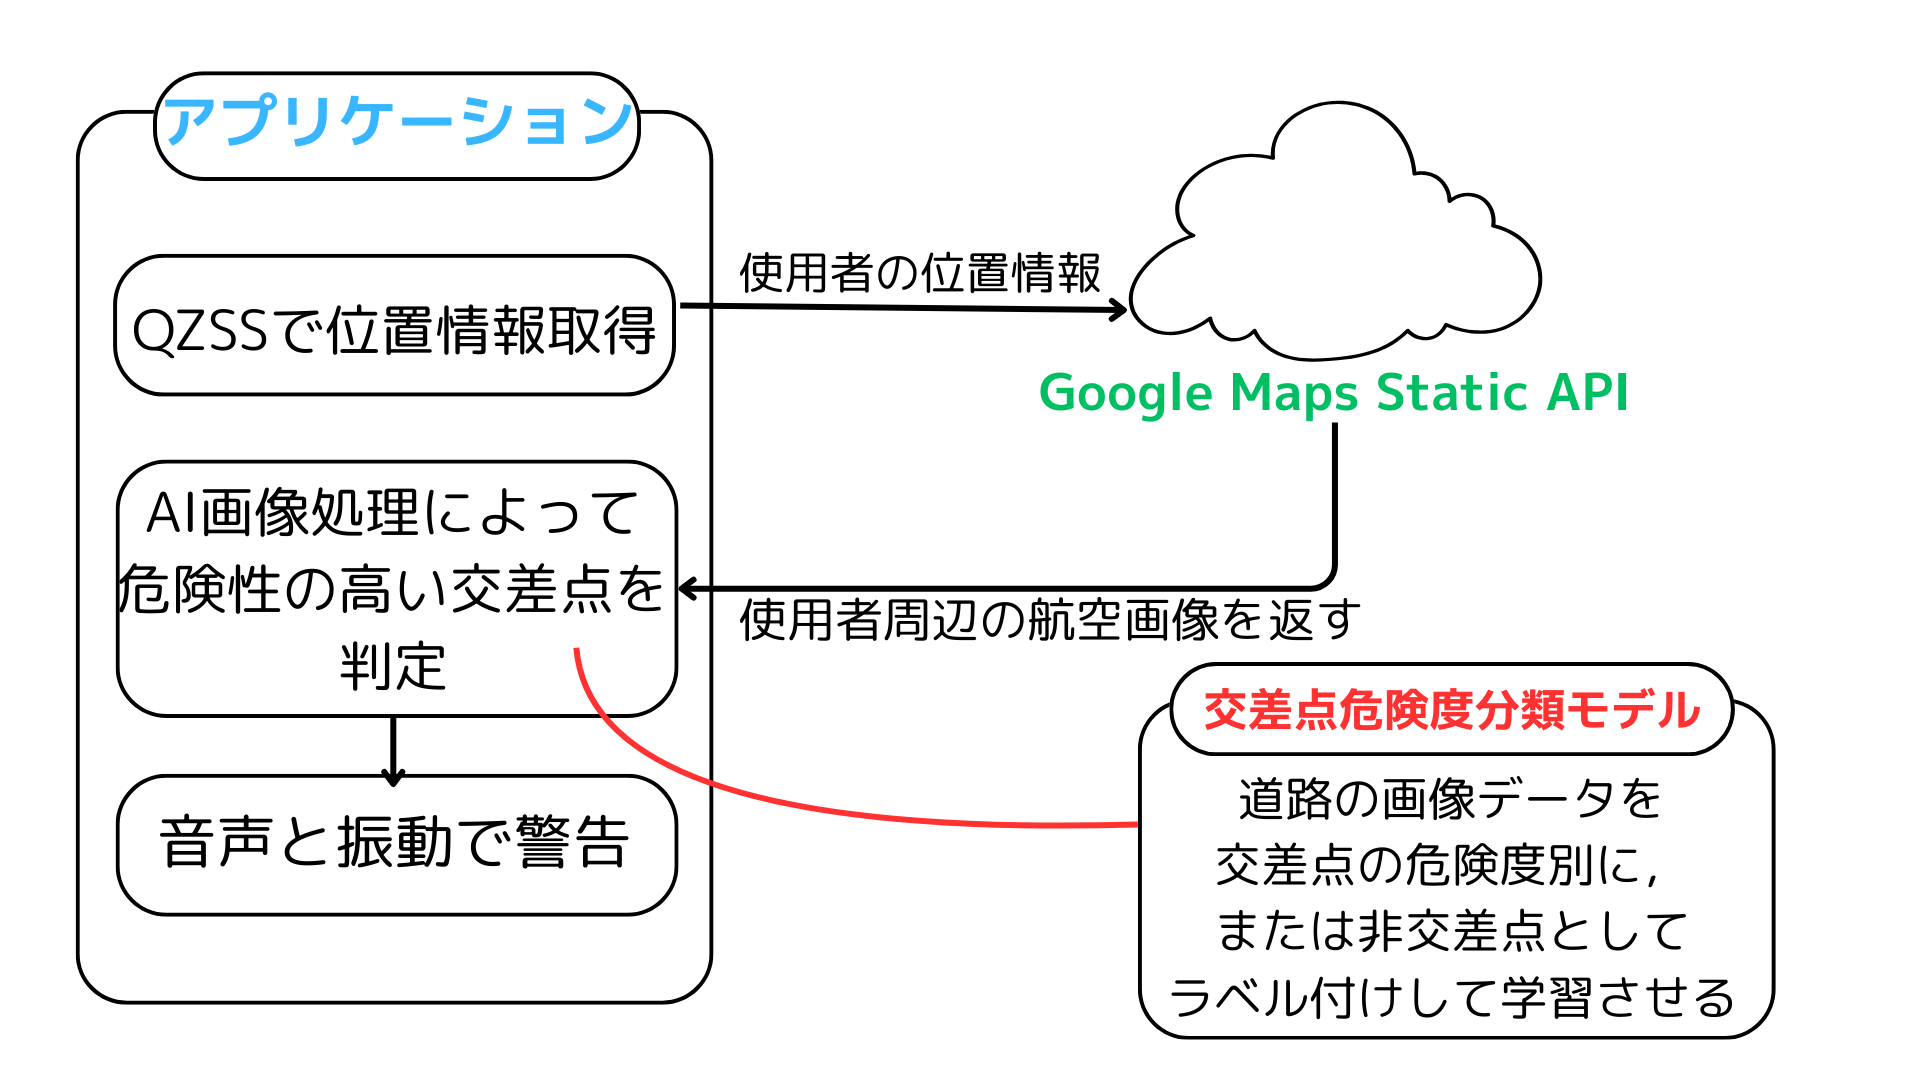
\includegraphics[width=14cm]{./Figs/system_new.png}
  \caption{危険交差点警告システムのシステム構成図}
  \label{fig:system}
\end{figure}

本システムの動作の流れを図\ref{fig:system}に示す.
まず,スマートフォンのQZSSから位置情報を取得する.
次に,Google Maps Static APIを用いて,現在地周辺の航空画像を取得する.

取得した航空画像は,事前に学習させた畳み込みニューラルネットワークによって処理され,道路の形状や障害物の配置などを解析し,交差点の有無と危険度を自動判定する.

危険性の高い交差点が検出された場合,搭乗者に対して音声とバイブレーションで警告される.
具体的には,スマートフォンから「危険な交差点があります.注意してください」といった警告が行われるとともに,
バイブレーション機能を用いて触覚的な警告も同時に行われる.

\section{提案手法の実現可能性の評価と妥当性の検証}

\subsection{主張・手法のまとめ}
本提案は,自転車搭乗者の注意力の限界を補い,出会い頭衝突の事故を防ぐための危険交差点警告システムである.
危険交差点警告システムでは,QZSSを用いて取得した使用者の位置情報を,Google Maps Static APIを用いることで現在地周辺の航空画像を取得し,
取得した航空画像をAIによる画像認識技術を用いて危険検知を行い,搭乗者に音声とバイブレーションで警告する.
このシステムにより,幅広い年齢層の自転車搭乗者の道路交通安全を守ることができると期待される.

\subsection{実現可能性の評価}
提案手法の実現可能性について評価する.
提案手法は,主にQZSSとGoogle Maps Static APIを用いて現在地周辺の航空画像を取得し,AIによる画像認識技術を用いて交差点を検出する.
これらの技術は,現在の技術水準で十分に実現可能である.

まず,Google Maps Static APIによる航空画像の取得の範囲について評価する.
本システムでは,zoomレベルを19に設定する.zoomレベルが19の場合,1ピクセルあたりの地上距離は$0.2986m$であり,
画像の取得範囲は,(4)のようになる\cite{ref:zoomrevel}.

\begin{align}
\mathrm{取得範囲(半径R)} = \frac{S\times m/px}{2} = \frac{640 \times 0.2986}{2} = \frac{191.104}{2} ≈ 95.55 \text{ m}
\end{align}

Google Maps Static APIを用いて取得できる航空画像の範囲は,現在地を中心に半径約95.55mとなる.
この範囲は,通常の自転車の走行速度約15km/hであれば,約14秒間隔で取得できるため,十分な頻度で航空画像を取得できる.

次に,AIによる画像認識技術の精度について評価する.
この評価には,あらかじめ「非交差点」「安全な交差点」「危険な交差点」の3クラスで人手でラベル付けされた航空画像データセットを用い,AIによる分類結果との一致度を確認する.

\begin{table}[H]
  \centering
  \caption{提案手法の評価指標}
  \label{tab:evaluation_metrics}
  \begin{tabular}{|c|c|}
    \hline
    指標 & 説明 \\ \hline
    Precision(各クラス) & 各クラスで正しく判定した割合 \\ \hline
    Recall(各クラス) & 各クラスの実際のデータを正しく判定した割合 \\ \hline
    F1スコア(各クラス) & PrecisionとRecallの調和平均 \\ \hline
    Macro平均 & 各クラスの指標の平均値 \\ \hline
    Accuracy & 全体の正解率 \\ \hline
  \end{tabular}
\end{table}

評価指標として,Precision,Recall,F1スコアを各クラスごとに算出し,その平均(Macro平均)とAccuracyを用いる.
各指標は(5)〜(9)の数式で表される.

\begin{align}
\mathrm{Accuracy} &= \frac{\sum_{i=1}^{N} TP_i}{\sum_{i=1}^{N} (TP_i + FP_i + FN_i)} \\
\mathrm{Precision}_i &= \frac{TP_i}{TP_i + FP_i} \\
\mathrm{Recall}_i &= \frac{TP_i}{TP_i + FN_i} \\
\mathrm{F1}_i &= 2 \cdot \frac{\mathrm{Precision}_i \cdot \mathrm{Recall}_i}{\mathrm{Precision}_i + \mathrm{Recall}_i} \\
\mathrm{Macro\text{-}F1} &= \frac{1}{N} \sum_{i=1}^{N} \mathrm{F1}_i
\end{align}

今回は,実際のデータが存在しないため,各指標の目標値を設定し,それをもとに本提案の実現可能性を評価する.
本システムでは各評価指標の目標値として,
Precision,Recall,F1スコア,Macro平均をそれぞれ0.8以上,Accuracyを0.85以上に設定する.
先行研究によれば,AIを用いた道路のセマンティックセグメンテーション技術は,走行可能領域の識別において約80\%から90\%の精度を達成している
\cite{ref:road_segmentation}.そのため,今回はこの先行研究を参考に,80\%と90\%の中間値である85\%をAccuracyの目標値とした.
また,この精度を実現するために約100エポックの学習が必要であると考えられる.
本システムの精度が目標値のように高ければ,より正確に危険な交差点を検出できるため,搭乗者に対して適切な警告を行うことが可能となる.
システムの精度が低いと,常に警告が作動したり逆に危険な交差点を見逃したりと,搭乗者からの信頼を失う可能性があり,危険な交差点を検出しても警告を無視される恐れがある.
しかし,高精度なシステムを実現できれば,不要な警告が減り警告への信頼性が高まるため,搭乗者は警告を真剣に受け止めるようになり,
安全行動を促すことができると考えられる.

ここまではシステムの精度について評価したが,ここでは警告によって搭乗者の行動がどのように変化するかについても考慮する.
歩行者のスマートフォン使用が原因の事故を防ぐための研究では,bluetoothビーコンを用いた警告システムによって,使用者の71\%がスマートフォンの使用を中止したと報告されている\cite{ref:user_alert}.
この先行研究を参考にここでは,システムが警告を発した際に、搭乗者が実際に減速や安全確認といった適切な行動をとる確率として,70\%を想定する.

上記の指標をもとに,危険な状況に対して本システムが有効に機能する確率(システムの有効率)は(10)のように計算できる.
\begin{align}
85\% (検知成功率) × 70\% (搭乗者の行動変容率) = 59.5\%
\end{align}
となる.出会い頭衝突による事故全体に対して本システムが適用されると仮定した場合,(10)より,出会い頭衝突の事故率を59.5\%削減させることが期待できる.

以上のことから,本システムは,現在の技術水準で十分に実現可能であり,提案手法の実現可能性は高いと評価できる.

\subsection{妥当性の検証}
提案手法の妥当性について説明する.
既存の交通事故多発エリア警告システムでは,事故データに依存することから,自動車の交通量が少ない地域では判定精度が低下する恐れがある点や突発的な道路状況の変化に対応できない点が問題であり,
事故データのみに偏った情報を基にしてしまうと,地域や環境に性能が左右されてしまうため,広範囲で適用できるとは限らないという問題が生じるため,より即時的で柔軟な危険検知が求められる.
しかし本システムは事故データに依存せず,AIを用いることでその場で危険を判定することができ,複雑な危険要因でも即時的な対応を可能とし,地域や環境に関係なくより広範囲での適用が可能となる.

本システムはスマートフォンアプリケーションとして実装するため,専用のハードウェアを必要とせず,既存のスマートフォンを活用することができるという点でも妥当性がある.
専用のハードウェアから開発すると,その分のコストと開発期間が大量にかかるが,本システムはスマートフォンアプリケーションとして実装する.
それに加え,スマートフォンの持つ高性能なCPU/GPU,GNSSモジュール,通信機能,そして豊富なセンサー群を最大限に活用できるため,効率的なシステム構築が可能である.
そのため本システムには,専用ハードウェアから開発するのに比べて,低コストで迅速に導入できるという点で優位性がある.
さらに,低コストであることから,インフラ整備といった大規模な投資が難しい地域でも導入が可能であり,より広範囲での適用が期待できる.

また,本提案では交差点の判定の際,過去の事故データではなく,航空画像を用いた.
第1節で述べたように,既存の自動車向け衝突防止システムADASは,警告や自動ブレーキによって使用者の安全を守るシステムとして知られているが,
先行研究では,衝突事故の事故事例の少なさから,有意な結果が得られなかった.
このように過去の事故データに依存してしまうと,データが不足している地域では効果が限定的になる可能性がある.
さらに,過去の事故データに基づくシステムは,新たな交通状況や未経験の事故パターンに対応できない可能性があり,より柔軟な適応が求められる.
しかし,本システムは過去の事故データに依存せず,航空画像を用いて危険な交差点を検出することは,地域や環境に関係なく,より広範囲での適用が可能である.

本システムはアルゴリズムではなくAIを用いているが,従来のアルゴリズムでは特定の条件に合致しない場合は検出できない事があり,
道路の広さだけでなく形状や道の勾配など無数の要因が絡み複雑になると,すべての要因を人間が分析してルール化することは非常に困難である.
しかし,AIは人間が言語化・ルール化しにくい複雑な特徴を,画像ピクセルのパターンから直接捉えることを得意としている.
そのため,定量的な判断ではなく定性的な判断を行うことにより,より柔軟に危険な交差点を検出できると考えられる.
また,今回は見通しの悪さを明確に定義したが,今回定義した要因以外にも,例えば交通量の多さや信号機の有無など,様々な要因が交差点の危険度に影響を与える可能性がある.
したがって,導入後も見通しの悪さの他の要因を追加して学習させることで,さらに複雑な要因が絡む交差点での危険検出が可能になると考えられる.

本提案は自転車搭乗者の行動変容を促すことを目的としているため,法令違反や不注意を完全に無くすことは難しいが,
自転車搭乗者に対して自動かつ適切な注意喚起を行うことで,事故のリスクを低減できると考える.

\section{おわりに}
\subsection{まとめ}
本提案では,自転車搭乗者の注意力の限界を補い,出会い頭衝突事故を防止するため,
従来のシステムより広範囲に適用でき柔軟に対応可能な「危険交差点警告システム」を,
AIによる画像認識技術を中核として提案した.

このシステムは,QZSSを用いて取得した使用者の位置情報をもとにGoogle Maps Static APIを用いて現在地周辺の航空画像を取得し,
取得した航空画像を畳み込みニューラルネットワーク(CNN)で画像処理することで,交差点のリアルタイムでの危険度分析・判定をする.
危険であると判定された場合,搭乗者に音声とバイブレーションで警告を行うことで,搭乗者に安全運転を促し,事故防止につなげる.
既存のスマートフォンを用いることで短期間かつ低コストで実装することができ,過去の事故データに依存しない危険分析が行えることで,
統計データの少ないまたは存在しない地域でも,高い汎用性と柔軟性が期待できる.

本システムの目標とする精度と搭乗者の行動変容率を考慮した結果,出会い頭衝突の事故率を約59.5\%削減させることが可能であると評価した.
そのため提案手法によって,出会い頭衝突による事故の発生率を約10\%削減させるという目標を達成することは可能であると考えられる.

\subsection{考察}
今回提案した「危険交差点警告システム」は,自転車搭乗者の安全運転を支援するための新しいアプローチである.
本提案では,AIによる危険の判定という方法を採用したが,固定のルールベースに基づいて判定を行う従来のアルゴリズムや,過去の統計に基づく手法と違い,視覚情報から
リアルタイムで直接的に危険の判定を行うことができるうえに,複雑な状況にも対応できることから,汎用性と柔軟性に優れている.

本システムはスマートフォンアプリケーションとして実装するため,専用のハードウェアを必要とせず,
ハードウェア開発にかかるコストや時間を大幅に削減できるという点でも優れている.また,リアルタイムの画像認識による危険度分析は,
交差点における無数に存在する危険的要因を捉えることができ,従来の手法では見逃されがちな危険な交差点も検出できる.
さらに,本システムでの警告手段として,光や画面表示などの視覚的警告ではなく,音声とバイブレーションを用いることで,
搭乗者は運転中に画面を見る必要がなく,光によって視界が遮られることもないため,運転を妨げることなく注意喚起が可能である.

航空画像取得のために用いたGoogle Maps Static APIは,同様に地図画像の取得が可能なGoogle Maps JavaScript APIと比較して,
ドキュメントが豊富であることと通信速度が高速であるのに加え,本提案では交差点の形状や障害物など静的な情報のみを取得すればよいため,
動的な地図表示が可能なGoogle Maps JavaScript APIよりも,静的な情報の取得に特化しているという利点がある.また,動的な地図表示を行う
ことにより,画面注視を促し安全性を損なう可能性もあるため,Google Maps JavaScript APIを使わない方が返って安全であると考えられる.

今後の課題としては,提案手法の実装と評価を行い,実際の使用環境においても高い精度で危険な交差点を検出できるようにすることが挙げられる.
同様に,システムの精度や搭乗者の行動変容率についても,調査によって実際の使用環境でのデータを収集し評価する必要があり,
実際の事故率の低下に寄与するかどうかを検証することが求められる.

\subsection{結論}
本レポートで提案した「危険交差点警告システム」は,自転車での出会い頭衝突の交通事故という重要な安全課題に対して,
AIによる画像認識技術と既存のモバイルデバイスを組み合わせることで,実用的かつ効果的な解決策を提供するものである.
本提案での航空画像を用いたリアルタイムの画像認識に基づいて危険を予測し,音声とバイブレーションで警告を行うシステムを利用することで,
従来の交通安全教育で補いきれなかった運転者の安全意識の形骸化の問題を補い,事故の事前防止に貢献できる.
これにより,子どもから高齢者まで,幅広い年齢層の自転車搭乗者の安全運転を支援し,交通事故の削減に寄与することが期待される.

第1節で掲げた目標である「出会い頭衝突による事故の発生率を約10\%削減させる」ことは,本システムの導入により,
達成できることが期待される.これは,令和6年中の自転車関連事故件数が67,531件であることから,約3,570件の事故削減に相当し,
自転車搭乗者の安全性向上に大きく寄与するものである.

今後の展望としては,時間帯や天候の変化に対応し,より多くの要因にも対応できるシステムにすることが挙げられる.
時間帯や天候の変化に対応するため,また判定精度を向上させるために,さらにデータを収集し汎用性を高めることが必要である.
また,本提案のシステムに,従来のシステムで用いられる事故データに基づく危険度分析を組み合わせることで,
リアルタイムに得られる物理的な危険性と,過去の統計的に裏付けられた危険性の両面から総合的な評価を行うことが可能となる.
これにより,実際に事故が多発している交差点では警告の優先度を高め,逆に事故データが少ない場所では不要な警告を抑制できるため,
利用者にとって説得力があり信頼性の高い警告システムとなることが期待される.

このような拡張を加えることで,本システムの実用性はさらに高まり,より多くの自転車搭乗者の安全確保に寄与できると考えられる.

\begin{thebibliography}{16}
\bibitem{ref:koutuusyou_1} 国土交通省, 「自転車活用推進計画」, \url{https://www.mlit.go.jp/road/bicycleuse/good-cycle-japan/assets/pdf/jitensha_katsuyo.pdf}.
\bibitem{ref:koutuusyou_2}  国土交通省, 「第1回自転車の活用推進に向けた有識者会議 自転車の活用に関する現状について」, \url{https://www.mlit.go.jp/road/ir/ir-council/bicycle-up/06pdf/02.pdf}.
\bibitem{ref:sonpo_1} 一般社団法人 日本損害保険協会, 「自転車の事故 〜安全な乗り方と事故への備え〜2024年8月版」, \url{https://www.sonpo.or.jp/report/publish/koutsu/g34l0i0000006z5o-att/book_bicycle2.pdf}.
\bibitem{ref:adas} Irene Isaksson Hellman, Magdalena Lindman, 「Estimating the crash reducing effect of Advanced Driver Assistance Systems (ADAS) for vulnerable road users」\url{https://tsr.international/TSR/article/view/25177/22639}
\bibitem{ref:adas_purpose} Vikram Maheshri, Clifford Winston, Yidi Wu, 「AI AT THE WHEEL:
THE EFFECTIVENESS OF ADVANCED DRIVER-ASSISTANCE SYSTEMS AND ITS IMPLICATIONS FOR POLICY」, \url{https://vmaheshri.github.io/files/papers/ADAS%20paper.pdf}
\bibitem{ref:qzss} 内閣府, 「準天頂衛星システム(みちびき)」, \url{https://qzss.go.jp/}.
\bibitem{ref:developer_static} Google, 「Google Maps Platform developer tools "Maps Static API"」, \url{https://developers.google.com/maps/documentation/maps-static/overview?hl=ja}.
\bibitem{ref:developer_js} Google, 「Google Maps Platform developer tools "Maps JavaScript API"」, \url{https://developers.google.com/maps/documentation/javascript/examples/map-simple}.
\bibitem{ref:bycicle} 岸田真, 「日本の自転車交通の現状と改善への取り組み」, \url{https://www.jice.or.jp/cms/kokudo/pdf/reports/act/20th/nikkan2009_05.pdf}
\bibitem{ref:responsibility} 内閣府, 「最高速度違反による交通事故対策検討会 中間報告書 第3章 最高速度違反による交通事故対策の効果等」, \url{https://www8.cao.go.jp/koutu/taisaku/max-speed/chukan/pdf/s4-1.pdf}
\bibitem{ref:brake_distance} 公益財団法人交通事故総合分析センター, 「速度による制動現象の差異と
速度による事故発生傾向の差異について」, \url{https://www.moj.go.jp/content/001421877.pdf}
\bibitem{ref:dry_road}Ali Abdi Kordani, Omid Rahmani, Amir Saman Abdollahzadeh Nasiri, Sid Mohammad Boroomandrad, 「Effect of Adverse Weather Conditions on Vehicle Braking
Distance of Highways」, \url{https://www.researchgate.net/publication/323000066_Effect_of_Adverse_Weather_Conditions_on_Vehicle_Braking_Distance_of_Highways/link/5a7bb6b20f7e9b55f65aba6d/download?_tp=eyJjb250ZXh0Ijp7ImZpcnN0UGFnZSI6Il9kaXJlY3QiLCJwYWdlIjoicHVibGljYXRpb24iLCJwcmV2aW91c1BhZ2UiOiJfZGlyZWN0In19}.
\bibitem{ref:newral} 内田祐介 山下隆義,「物体認識のための畳み込みニューラルネットワークの研究動向」,\url{https://search.ieice.org/bin/pdf_link.php?category=D&lang=J&year=2019&fname=j102-d_3_203&abst=}
\bibitem{ref:cnn_vit} Zhiying Lu, Hongtao Xie, Chuanbin Liu, Yongdong Zhang, 「Bridging the Gap Between Vision Transformers and
Convolutional Neural Networks on Small Datasets」, \url{https://proceedings.nips.cc/paper_files/paper/2022/file/5e0b46975d1bfe6030b1687b0ada1b85-Paper-Conference.pdf}.
\bibitem{ref:zoomrevel}
Microsoft,「Zoom levels and tile grid」,\url{https://learn.microsoft.com/en-us/azure/azure-maps/zoom-levels-and-tile-grid?tabs=csharp}
\bibitem{ref:road_segmentation}
Zhaoxiang Wang, Kaiqi Huang, 「Road Scene Semantic Segmentation Based on Deep Learning」, 2023.
\bibitem{ref:user_alert}
Raiful Hasan, Mohammad Aminul Hoque, Yasser Karim, Russell Griffin, David C. Schwebel, Ragib Hasan「Someone to Watch Over You: Using Bluetooth Beacons for Alerting Distracted Pedestrians」\url{https://pmc.ncbi.nlm.nih.gov/articles/PMC9696539/#S30}
\end{thebibliography}

\end{document}